%!TEX program = xelatex
%!TEX encoding = UTF-8
\documentclass[12pt]{report}
\usepackage{caption}
\usepackage{amssymb}
\usepackage{amsmath,amsfonts,amsthm,amstext}
\usepackage[brazil]{babel}
% \usepackage[latin1]{inputenc}
\usepackage{graphicx}
\graphicspath{{/home/jfreitas/GitHub/Emural_Moodle/imagens/}}
\usepackage{enumerate}
\usepackage{hyperref}
\usepackage{float}
\usepackage{fancyhdr}
\def\email{jfreitas@mat.unb.br}

\def\ano{2023}
\def\semestre{1}
% \setlength{\topmargin}{-1.0in}
% \setlength{\oddsidemargin}{0in}
% \setlength{\textheight}{10.1in}
% \setlength{\textwidth}{6.5in}
% \setlength{\baselineskip}{12mm}

\pagestyle{fancy}

\begin{document}

\begin{center}
{\Large \textbf{Tutorial para gerar lista de presença para o E-mural e o MoodleMAT}}
\end{center}
\vspace{.3cm}
\hrule

\vspace{.7cm}

Após fazer o login no SIGAA entre na sua disciplina. Em seguida faça o seguinte:

\begin{enumerate}[\bf 1)]
    \item No lado esquerdo da tela procure a opção ``Diário Eletrônico'' e clique nela.
	\begin{figure}[H]
    	\centering
    	\hspace*{-2.5cm}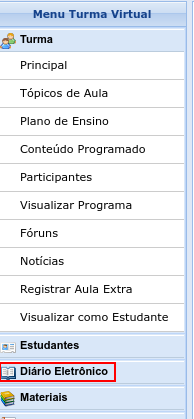
\includegraphics[width = .4\columnwidth]{diario_eletronico.png}
  	\end{figure}

	\newpage

        \item Na tela que se abre procure a opção ``Lista de Presença'' e clique nela.
	\begin{figure}[H]
	   \centering
        	\hspace*{-2.5cm}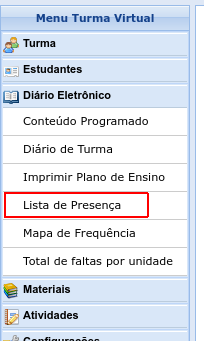
\includegraphics[width = 0.4\columnwidth]{lista_presenca.png}
	    \end{figure}

	\item Ao clicar nessa opção o arquivo da lista de presença será salvo no computador. Envie esse arquivo PDF para o e-mail: \href{mailto:{\email}}{\email}.
    \end{enumerate}
\end{document}
